\documentclass{standalone}
\usepackage{tikz}
\usetikzlibrary{patterns, positioning}
\usepackage[sfdefault]{ClearSans} %% option 'sfdefault' activates Clear Sans as the default text font
\usepackage[T1]{fontenc}

\begin{document}
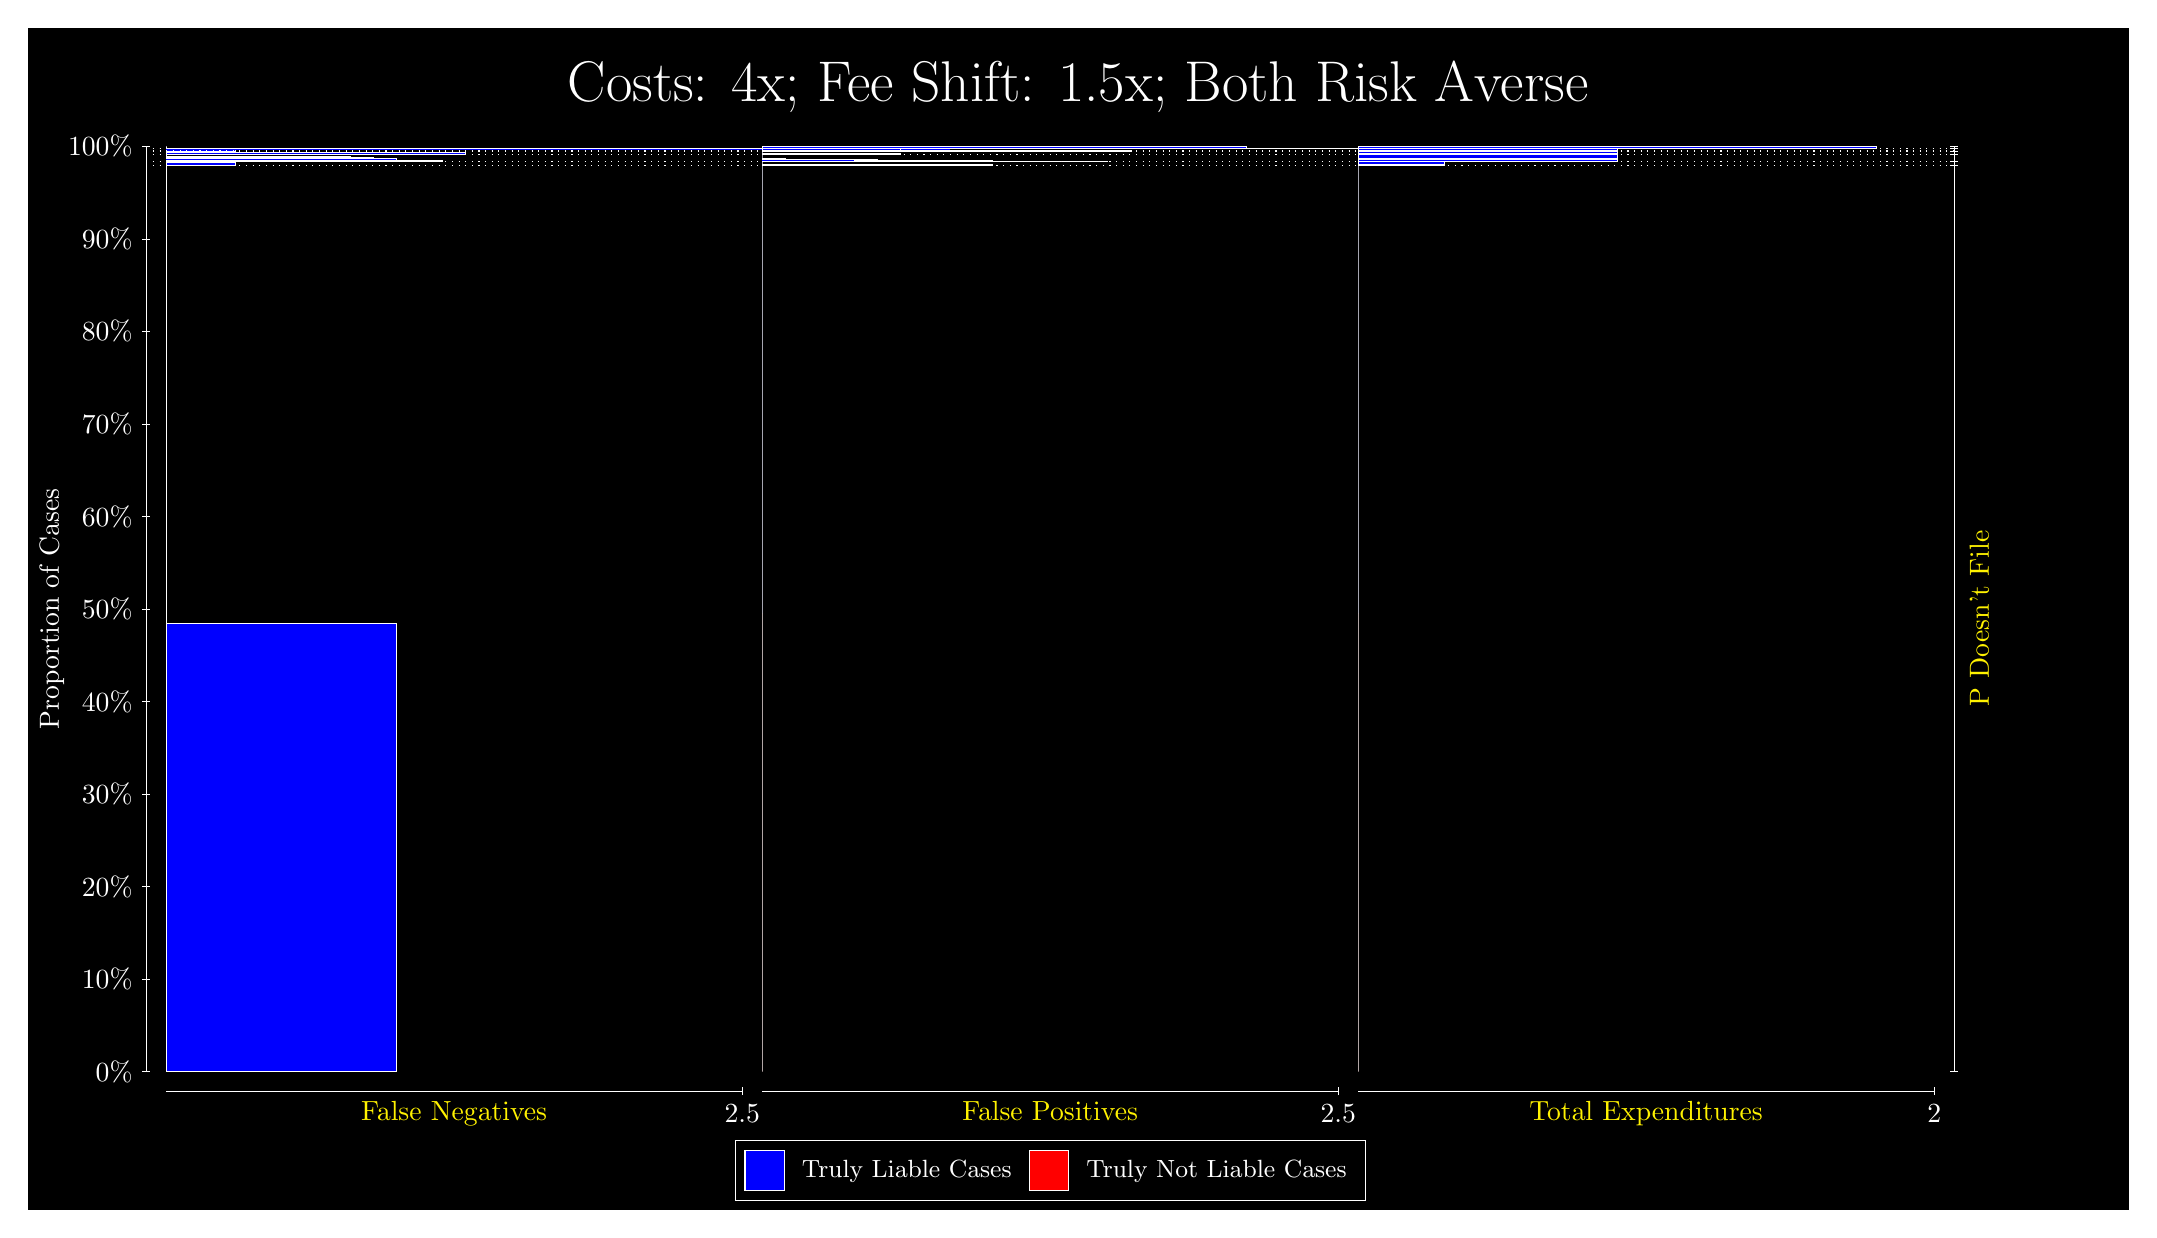
\begin{tikzpicture}
\draw[fill=black] (0,0) rectangle (26.667,15);
\draw[text=white] (0,13.5) rectangle (26.667,15) node[midway] {\huge Costs: 4x; Fee Shift: 1.5x; Both Risk Averse};
\draw[white, very thin] (1.5,1.75) -- (1.5,13.5);
\node[rotate=90, text=white, anchor=center] at (0.3, 7.625) {Proportion of Cases};
\draw[white, very thin] (1.45,1.75) -- (1.55,1.75);
\node[text=white, anchor=east] at (1.45, 1.75) {0\%};
\draw[white, very thin] (1.45,2.925) -- (1.55,2.925);
\node[text=white, anchor=east] at (1.45, 2.925) {10\%};
\draw[white, very thin] (1.45,4.1) -- (1.55,4.1);
\node[text=white, anchor=east] at (1.45, 4.1) {20\%};
\draw[white, very thin] (1.45,5.275) -- (1.55,5.275);
\node[text=white, anchor=east] at (1.45, 5.275) {30\%};
\draw[white, very thin] (1.45,6.45) -- (1.55,6.45);
\node[text=white, anchor=east] at (1.45, 6.45) {40\%};
\draw[white, very thin] (1.45,7.625) -- (1.55,7.625);
\node[text=white, anchor=east] at (1.45, 7.625) {50\%};
\draw[white, very thin] (1.45,8.8) -- (1.55,8.8);
\node[text=white, anchor=east] at (1.45, 8.8) {60\%};
\draw[white, very thin] (1.45,9.975) -- (1.55,9.975);
\node[text=white, anchor=east] at (1.45, 9.975) {70\%};
\draw[white, very thin] (1.45,11.15) -- (1.55,11.15);
\node[text=white, anchor=east] at (1.45, 11.15) {80\%};
\draw[white, very thin] (1.45,12.325) -- (1.55,12.325);
\node[text=white, anchor=east] at (1.45, 12.325) {90\%};
\draw[white, very thin] (1.45,13.5) -- (1.55,13.5);
\node[text=white, anchor=east] at (1.45, 13.5) {100\%};

\draw[white, very thin] (24.457,1.75) -- (24.457,13.5);
\draw[white, very thin] (24.407,1.75) -- (24.507,1.75);
\node[anchor=west] at (24.407, 1.75) {};
\draw[white, very thin] (24.407,13.259) -- (24.507,13.259);
\node[anchor=west] at (24.407, 13.259) {};
\draw[white, very thin] (24.407,13.311) -- (24.507,13.311);
\node[anchor=west] at (24.407, 13.311) {};
\draw[white, very thin] (24.407,13.397) -- (24.507,13.397);
\node[anchor=west] at (24.407, 13.397) {};
\draw[white, very thin] (24.407,13.44) -- (24.507,13.44);
\node[anchor=west] at (24.407, 13.44) {};
\draw[white, very thin] (24.407,13.469) -- (24.507,13.469);
\node[anchor=west] at (24.407, 13.469) {};
\draw[white, very thin] (24.407,13.477) -- (24.507,13.477);
\node[anchor=west] at (24.407, 13.477) {};
\draw[white, very thin] (24.407,13.5) -- (24.507,13.5);
\node[anchor=west] at (24.407, 13.5) {};

\draw[white, very thin, fill=blue] (1.75,1.75) rectangle (4.6775,7.4385);
\draw[white, very thin, fill=red] (1.75,7.4385) rectangle (1.75,13.259);
\draw[white, very thin, fill=blue] (1.75,13.259) rectangle (2.6283,13.299);
\draw[white, very thin, fill=red] (1.75,13.299) rectangle (1.75,13.311);
\draw[white, very thin, fill=blue] (1.75,13.311) rectangle (5.2631,13.321);
\draw[white, very thin, fill=blue] (1.75,13.321) rectangle (4.9703,13.324);
\draw[white, very thin, fill=blue] (1.75,13.324) rectangle (4.6775,13.342);
\draw[white, very thin, fill=blue] (1.75,13.342) rectangle (4.3848,13.343);
\draw[white, very thin, fill=blue] (1.75,13.343) rectangle (4.3848,13.358);
\draw[white, very thin, fill=blue] (1.75,13.358) rectangle (4.092,13.374);
\draw[white, very thin, fill=blue] (1.75,13.374) rectangle (3.7993,13.376);
\draw[white, very thin, fill=blue] (1.75,13.376) rectangle (3.5065,13.377);
\draw[white, very thin, fill=blue] (1.75,13.377) rectangle (3.2138,13.378);
\draw[white, very thin, fill=blue] (1.75,13.378) rectangle (2.921,13.379);
\draw[white, very thin, fill=red] (1.75,13.379) rectangle (1.75,13.397);
\draw[white, very thin, fill=blue] (1.75,13.397) rectangle (5.5558,13.429);
\draw[white, very thin, fill=red] (1.75,13.429) rectangle (1.75,13.44);
\draw[white, very thin, fill=blue] (1.75,13.44) rectangle (2.6283,13.463);
\draw[white, very thin, fill=red] (1.75,13.463) rectangle (1.75,13.469);
\draw[white, very thin, fill=blue] (1.75,13.469) rectangle (11.704,13.472);
\draw[white, very thin, fill=red] (1.75,13.472) rectangle (1.75,13.477);
\draw[white, very thin, fill=red] (1.75,13.477) rectangle (1.75,13.48);
\draw[white, very thin, fill=blue] (1.75,13.48) rectangle (1.75,13.5);
\draw[white, very thin, fill=red] (9.3189,1.75) rectangle (9.3189,7.5709);
\draw[white, very thin, fill=blue] (9.3189,7.5709) rectangle (9.3189,13.259);
\draw[white, very thin, fill=red] (9.3189,13.259) rectangle (12.246,13.272);
\draw[white, very thin, fill=blue] (9.3189,13.272) rectangle (9.3189,13.311);
\draw[white, very thin, fill=red] (9.3189,13.311) rectangle (13.71,13.312);
\draw[white, very thin, fill=red] (9.3189,13.312) rectangle (13.417,13.312);
\draw[white, very thin, fill=red] (9.3189,13.312) rectangle (13.125,13.312);
\draw[white, very thin, fill=red] (9.3189,13.312) rectangle (12.832,13.313);
\draw[white, very thin, fill=red] (9.3189,13.313) rectangle (12.539,13.316);
\draw[white, very thin, fill=red] (9.3189,13.316) rectangle (12.246,13.32);
\draw[white, very thin, fill=red] (9.3189,13.32) rectangle (11.954,13.325);
\draw[white, very thin, fill=red] (9.3189,13.325) rectangle (11.661,13.326);
\draw[white, very thin, fill=red] (9.3189,13.326) rectangle (11.368,13.329);
\draw[white, very thin, fill=blue] (9.3189,13.329) rectangle (10.783,13.33);
\draw[white, very thin, fill=blue] (9.3189,13.33) rectangle (10.49,13.331);
\draw[white, very thin, fill=blue] (9.3189,13.331) rectangle (10.197,13.333);
\draw[white, very thin, fill=blue] (9.3189,13.333) rectangle (9.9044,13.334);
\draw[white, very thin, fill=blue] (9.3189,13.334) rectangle (9.6116,13.351);
\draw[white, very thin, fill=blue] (9.3189,13.351) rectangle (9.3189,13.397);
\draw[white, very thin, fill=red] (9.3189,13.397) rectangle (11.075,13.407);
\draw[white, very thin, fill=blue] (9.3189,13.407) rectangle (9.3189,13.44);
\draw[white, very thin, fill=red] (9.3189,13.44) rectangle (14.003,13.445);
\draw[white, very thin, fill=blue] (9.3189,13.445) rectangle (11.075,13.469);
\draw[white, very thin, fill=red] (9.3189,13.469) rectangle (9.3189,13.474);
\draw[white, very thin, fill=blue] (9.3189,13.474) rectangle (9.3189,13.477);
\draw[white, very thin, fill=red] (9.3189,13.477) rectangle (18.394,13.48);
\draw[white, very thin, fill=blue] (9.3189,13.48) rectangle (15.467,13.5);
\draw[white, very thin, fill=red] (16.888,1.75) rectangle (16.888,7.5709);
\draw[white, very thin, fill=blue] (16.888,7.5709) rectangle (16.888,13.259);
\draw[white, very thin, fill=red] (16.888,13.259) rectangle (17.986,13.272);
\draw[white, very thin, fill=blue] (16.888,13.272) rectangle (17.986,13.311);
\draw[white, very thin, fill=red] (16.888,13.311) rectangle (20.181,13.315);
\draw[white, very thin, fill=blue] (16.888,13.315) rectangle (20.181,13.331);
\draw[white, very thin, fill=red] (16.888,13.331) rectangle (20.181,13.333);
\draw[white, very thin, fill=blue] (16.888,13.333) rectangle (20.181,13.337);
\draw[white, very thin, fill=red] (16.888,13.337) rectangle (20.181,13.35);
\draw[white, very thin, fill=blue] (16.888,13.35) rectangle (20.181,13.397);
\draw[white, very thin, fill=red] (16.888,13.397) rectangle (20.181,13.407);
\draw[white, very thin, fill=blue] (16.888,13.407) rectangle (20.181,13.44);
\draw[white, very thin, fill=red] (16.888,13.44) rectangle (20.181,13.445);
\draw[white, very thin, fill=blue] (16.888,13.445) rectangle (20.181,13.469);
\draw[white, very thin, fill=red] (16.888,13.469) rectangle (23.475,13.474);
\draw[white, very thin, fill=blue] (16.888,13.474) rectangle (23.475,13.477);
\draw[white, very thin, fill=red] (16.888,13.477) rectangle (23.475,13.48);
\draw[white, very thin, fill=blue] (16.888,13.48) rectangle (23.475,13.5);
\draw[white, dotted] (1.5,13.259) -- (24.457,13.259);
\draw[white, dotted] (1.5,13.311) -- (24.457,13.311);
\draw[white, dotted] (1.5,13.397) -- (24.457,13.397);
\draw[white, dotted] (1.5,13.44) -- (24.457,13.44);
\draw[white, dotted] (1.5,13.469) -- (24.457,13.469);
\draw[white, dotted] (1.5,13.477) -- (24.457,13.477);
\draw[white, very thin] (1.75,1.5) -- (9.0689,1.5);
\node[text=yellow, anchor=north] at (5.4094, 1.5) {False Negatives};
\draw[white, very thin] (9.0689,1.45) -- (9.0689,1.55);
\node[text=white, anchor=north] at (9.0689, 1.45) {2.5};

\draw[white, very thin] (9.3189,1.5) -- (16.638,1.5);
\node[text=yellow, anchor=north] at (12.978, 1.5) {False Positives};
\draw[white, very thin] (16.638,1.45) -- (16.638,1.55);
\node[text=white, anchor=north] at (16.638, 1.45) {2.5};

\draw[white, very thin] (16.888,1.5) -- (24.207,1.5);
\node[text=yellow, anchor=north] at (20.547, 1.5) {Total Expenditures};
\draw[white, very thin] (24.207,1.45) -- (24.207,1.55);
\node[text=white, anchor=north] at (24.207, 1.45) {2};

\node[text=yellow, centered, rotate=90] at (24.777, 7.5047) {P Doesn't File};







\draw (12.978300999999998,1.5) node[draw=none] (baseCoordinate) {};
\begin{scope}[align=center]
        \matrix[scale=0.5, draw=white, below=0.5cm of baseCoordinate, nodes={draw}, column sep=0.1cm]{
            \node[rectangle, draw, minimum width=0.5cm, minimum height=0.5cm, fill=blue] {}; &
            \node[draw=none, font=\small, text=white] (B) {Truly Liable Cases}; &
            \node[rectangle, draw, minimum width=0.5cm, minimum height=0.5cm, fill=red] {}; &
            \node[draw=none, font=\small, text=white] (B) {Truly Not Liable Cases}; \\
            };
\end{scope}

\end{tikzpicture}
\end{document}